\documentclass[border=10pt,multi,tikz]{standalone}
\usepackage{tikz}
\usetikzlibrary{mindmap}
\pagestyle{empty}
\begin{document}
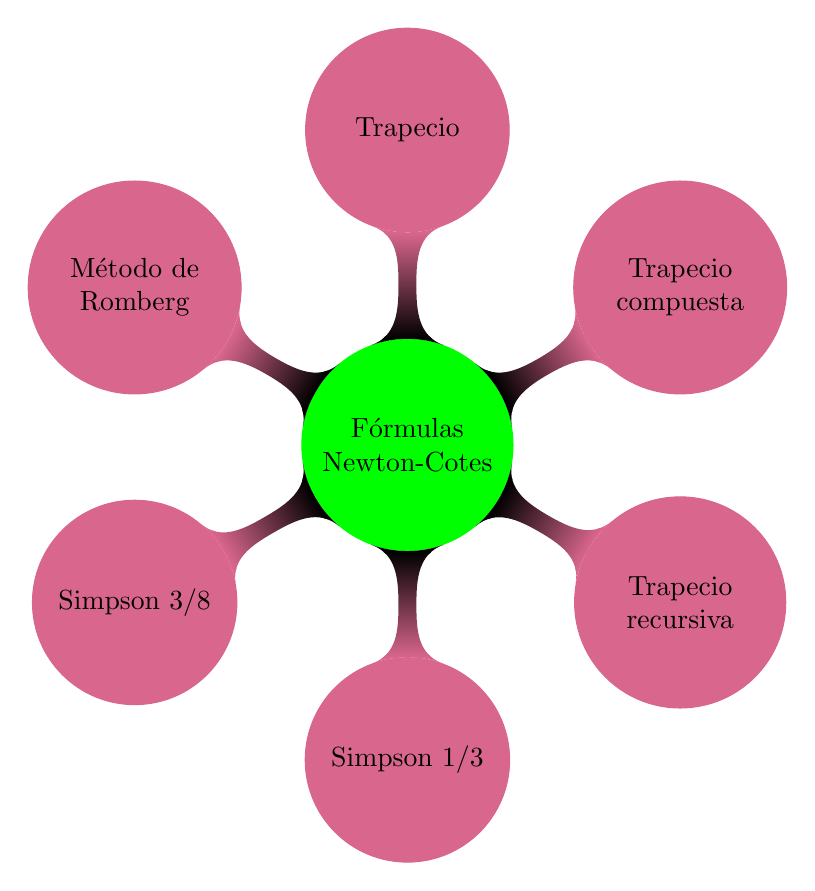
\begin{tikzpicture}[grow cyclic, text width=2.3cm, align=flush center, every node/.style={concept}, concept color=purple!60, 
    level 1/.style={level distance=4cm,sibling angle=60}]
    \node[concept color=green, level distance=5cm] {Fórmulas Newton-Cotes} [clockwise from=90]
        child { node {Trapecio}}
        child { node {Trapecio compuesta}}
        child { node {Trapecio recursiva}}
        child { node {Simpson $1/3$}}
        child { node {Simpson $3/8$}}
        child { node {Método de Romberg}}
    
    % child[concept color=pink!60!red, level distance= 5cm, sibling angle=120] { node {Fórmulas Gaussianas}
    %     child[rotate=-90] {node {Polinomios ortogonales}}
    % }
;
\end{tikzpicture}
\end{document}